\documentclass[10pt,aspectratio=169]{beamer}

% silence some Metropolis warnings
\usepackage{silence}
\WarningFilter{beamerthememetropolis}{You need to compile with XeLaTeX or LuaLaTeX}
\WarningFilter{latexfont}{Font shape}
\WarningFilter{latexfont}{Some font}

% define custom colors
\usepackage{xcolor}
\definecolor{dark gray}{HTML}{444444}
\definecolor{light gray}{HTML}{777777}
\definecolor{dark red}{HTML}{BB0000}
\definecolor{dark green}{HTML}{00BB00}
\definecolor{RoyalBlue}{cmyk}{1, 0.50, 0, 0}

% configure metropolis
\usetheme[numbering=fraction]{metropolis}
\setbeamercolor{background canvas}{bg=white}
\setbeamercolor{frametitle}{bg=dark gray}
\setbeamercolor{alerted text}{fg=dark red}
\setbeamercolor{item projected}{bg=dark red}
\setbeamercolor{local structure}{fg=dark red}
\setbeamersize{text margin left=0.5cm,text margin right=0.5cm}
\setbeamercovered{transparent=10}

% use thicker lines
\makeatletter
\setlength{\metropolis@titleseparator@linewidth}{1pt}
\setlength{\metropolis@progressonsectionpage@linewidth}{1pt}
\makeatother

% custom bullet points
\setbeamertemplate{itemize item}{\color{dark red}$\blacktriangleright$}
\setbeamertemplate{itemize subitem}{\color{dark red}$\blacktriangleright$}
\setbeamertemplate{itemize subsubitem}{\color{dark red}$\blacktriangleright$}
\newcommand{\custombullet}{{\color{dark red}$\blacktriangleright$}\hspace{0.5em}}


% imports
\usepackage[english]{babel}
\usepackage[utf8]{inputenc}
\usepackage{amsthm}
\usepackage{amssymb}
\usepackage{amsmath}
\usepackage{amsfonts}
\usepackage{mathtools}
\usepackage{mathabx}
\usepackage{stmaryrd}
\usepackage{graphicx}
\usepackage{hyperref}
\usepackage{xfrac}
\usepackage{appendixnumberbeamer}
\usepackage{tabularx}
\usepackage{listings}

% for code formatting
   \lstset{language=R,
           basicstyle=\ttfamily\scriptsize,
           keywordstyle=\color{blue}\ttfamily,
           stringstyle=\color{red}\ttfamily,
           commentstyle=\color{green}\ttfamily,
          breaklines=true
          }



% check and x marks
\usepackage{pifont}
\newcommand{\cmark}{{\color{dark green}\ding{51}}\hspace{0.3em}}
\newcommand{\xmark}{{\color{dark red}\ding{55}}\hspace{0.5em}}


% use classic font for math
\usepackage[T1]{fontenc} % Needed for Type1 Concrete \usepackage{concmath}
\usefonttheme{serif}
\usefonttheme{professionalfonts}
\usepackage{concmath}
\setbeamerfont{equation}{size=\tiny}



% diagrams
\usepackage{tikz}
\usetikzlibrary{decorations.pathreplacing, arrows, shapes, patterns, angles, quotes}

% references
\usepackage[natbibapa]{apacite}
\bibliographystyle{apacite}
\renewcommand{\bibsection}{}

% use ampersands instead of "and" for text citations
\AtBeginDocument{\renewcommand{\BBAB}{\&}}

% possessive cites
\makeatletter
\patchcmd{\NAT@test}{\else \NAT@nm}{\else \NAT@nmfmt{\NAT@nm}}{}{}
\DeclareRobustCommand\citepos
  {\begingroup
   \let\NAT@nmfmt\NAT@posfmt
   \NAT@swafalse\let\NAT@ctype\z@\NAT@partrue
   \@ifstar{\NAT@fulltrue\NAT@citetp}{\NAT@fullfalse\NAT@citetp}}
\let\NAT@orig@nmfmt\NAT@nmfmt
\def\NAT@posfmt#1{\NAT@orig@nmfmt{#1's}}
\makeatother

% spaced-out lists
\newenvironment{wideitemize}{\itemize\addtolength{\itemsep}{10pt}}{\enditemize}
\newenvironment{wideenumerate}{\enumerate\addtolength{\itemsep}{10pt}}{\endenumerate}

% replace footnotes with buttons
\usepackage[absolute,overlay]{textpos}
\newcounter{beamerpausessave}
\newcommand{\always}[1]{
    \setcounter{beamerpausessave}{\value{beamerpauses}}
    \setcounter{beamerpauses}{0}
    \pause
    #1 
    \setcounter{beamerpauses}{\value{beamerpausessave}}
    \addtocounter{beamerpauses}{-1}
    \pause
}
\newcommand{\buttons}[1]{\always{
    \begin{textblock*}{\paperwidth}(0.015\textwidth, 1.022\textheight)
        \scriptsize
        #1
    \end{textblock*}
}}
\newcommand{\appendixbuttons}[1]{\always{
    \begin{textblock*}{\paperwidth}(0.015\textwidth, 1.043\textheight)
        \scriptsize
        #1
    \end{textblock*}
}}
\newcommand{\goto}[2]{\hyperlink{#1}{{\color{dark red}$\smalltriangleright$} #2}\hspace{0.5em}}
\newcommand{\goback}[2]{\hyperlink{#1}{{\color{dark red}$\smalltriangleleft$} #2}\hspace{0.5em}}

% custom appendix
\renewcommand{\appendixname}{\texorpdfstring{\translate{Appendix}}{Appendix}}

% change color of cites and URLs
\let\oldcite\cite
\let\oldcitet\citet
\let\oldcitep\citep
\let\oldcitepos\citepos
\let\oldcitetalias\citetalias
\let\oldcitepalias\citepalias
\let\oldurl\url
\def\cite#1#{\citeaux{#1}}
\def\citet#1#{\citetaux{#1}}
\def\citep#1#{\citepaux{#1}}
\def\citepos#1#{\citeposaux{#1}}
\def\citetalias#1#{\citetaliasaux{#1}}
\def\citepalias#1#{\citepaliasaux{#1}}
\def\url#1#{\urlaux{#1}}
\newcommand*\citeaux[2]{{\color{light gray}\oldcite#1{#2}}}
\newcommand*\citetaux[2]{{\color{light gray}\oldcitet#1{#2}}}
\newcommand*\citepaux[2]{{\color{light gray}\oldcitep#1{#2}}}
\newcommand*\urlaux[2]{{\color{light gray}\oldurl#1{#2}}}
\newcommand*\citeposaux[2]{{\color{light gray}\oldcitepos#1{#2}}}
\newcommand*\citetaliasaux[2]{{\color{light gray}\oldcitetalias#1{#2}}}
\newcommand*\citepaliasaux[2]{{\color{light gray}\oldcitepalias#1{#2}}}

% custom math commands
\DeclareMathOperator*{\argmax}{argmax}
\DeclareMathOperator*{\argmin}{argmin}
\renewcommand{\Pr}{\mathbb{P}}
\newcommand{\E}{\mathbb{E}}
\newcommand{\Var}{\mathbb{V}}
\newcommand{\Cov}{\mathbb{C}}
\newcommand{\overbar}[1]{\mkern 1.5mu\overline{\mkern-1.5mu#1\mkern-1.5mu}\mkern 1.5mu}
\newcommand{\abs}[1]{\lvert#1\rvert}
\newcommand{\norm}[1]{\lVert#1\rVert}

% tables
\usepackage{booktabs}
\usepackage{colortbl}
\usepackage{multirow}
\usepackage{makecell}
\arrayrulecolor{dark red}

% custom date
\usepackage{datetime}
\newdateformat{monthyeardate}{\monthname[\THEMONTH] \THEYEAR}

% fix pauses with graphics
\usepackage{../resources/fixpauseincludegraphics}

% \documentclass[english,xcolor={dvipsnames},aspectratio=169]{beamer}
% \usepackage[italic]{mathastext}

% \usepackage{float}
% \usepackage{amsmath}
% \usepackage{amssymb}
% \usepackage{graphicx}
% \usepackage{setspace}
% \usepackage[outdir=./]{epstopdf}
% \usepackage{listings}

% \usepackage{caption,subcaption}
% \usepackage{booktabs}
% \usepackage[flushleft]{threeparttable}

% \usepackage{hyperref}
% \hypersetup{
%     colorlinks=true,
%     linkcolor=blue,
%     filecolor=magenta,      
%     urlcolor=blue,
% }

% \lstset{language=R,
%         basicstyle=\ttfamily\scriptsize,
%         keywordstyle=\color{blue}\ttfamily,
%         stringstyle=\color{red}\ttfamily,
%         commentstyle=\color{green}\ttfamily,
%        breaklines=true
% }


% \DeclareFontShape{OT1}{cmss}{b}{n}{<->ssub * cmss/bx/n}{} 
% \DeclareMathOperator*{\plim}{plim}

% \usepackage{siunitx}
% \sisetup{
% input-symbols = {()},
% group-digits  = false,
% explicit-sign
% }

% %\usetheme{CambridgeUS}
% \usetheme{Boadilla}
% \usecolortheme{seahorse}

% \setbeamertemplate{itemize subsubitem}{\tiny\raise1.5pt\hbox{\donotcoloroutermaths$\blacktriangleright$}}


% \usepackage{tikz}
% \usepackage{pgfplots}
% \pgfplotsset{compat=1.7}
% \usetikzlibrary{arrows, shapes, snakes, patterns, angles, quotes}

% \makeatletter


% \usepackage{setspace}
% \usepackage[normalem]{ulem}
% \setbeamersize{text margin left=5pt,text margin right=5pt}

% \makeatother

% \usepackage{babel}
\begin{document}

\pgfmathdeclarefunction{gauss}{2}{%
  \pgfmathparse{1/(#2*sqrt(2*pi))*exp(-((x-#1)^2)/(2*#2^2))}%
}

\title{Econometrics I}
\subtitle{Lecture 2: Asymptotic Statistics}

\author{Chris Conlon \\NYU Stern}
\date{Fall 2025}
\maketitle


\begin{frame}{Roadmap}
\begin{enumerate}
	\item Sample and population means
	\item Convergence in probability
	\item Law of Large Numbers
	\item Convergence in distribution
	\item Central Limit Theorem
\end{enumerate}
\end{frame}

\begin{frame}{Convergence}
\begin{itemize}
	\item Consider a sequence of numbers $\{X_i\}_{i=1}^n = \left(X_1,X_2,\ldots,X_n\right)$.
	\begin{itemize}
		\item Often people write $X_n =  \{X_i\}_{i=1}^n$ but I hate this.
	\end{itemize}
	\item We can ask what happens to some function $g(\{X_i\}_{i=1}^n)$ as $n \rightarrow \infty$.
	\begin{itemize}
		\item Simple Example: $X_i = \frac{1}{2^i}$ and $g(\cdot)$ is the summation so that $\lim_{n \rightarrow \infty}\sum_{i=1}^n \frac{1}{2^i} =  \frac{1}{2} + \frac{1}{4} + \frac{1}{8} + \cdots \rightarrow 1$.
	\end{itemize}
	\item Sequences of \alert{random variables} "approach" something too (other \alert{random variables})
	\item But what does \alert{approaching} mean?
\end{itemize}
\end{frame}

\begin{frame}{Convergence}
Let's define $S_n = g( \{X_i\}_{i=1}^n)$ as some \alert{statistic} of the sequence of random variables $\{X_i\}_{i=1}^n$.\\
 For example:
\begin{itemize}
	\item Summation: $S_n = \sum_{i=1}^n X_i$; Sample Average: $S_n = \frac{1}{n}\sum_{i=1}^n X_i$;
	\item Largest Element: $S_n = \max  X_i$
	\item Variance: $Var(X_1,X_2,\ldots,X_n)$.
	\item Something complicated: $X_1 - 2 X_2 + 3 X_3 - 4 X_4 \ldots$.
\end{itemize}
But our statistic could just be the identity function $S_n = \{X_i\}_{i=1}^n$ or transform $S_n = \{a X_i +b\}_{i=1}^n$ 
\end{frame}



\begin{frame}{Convergence in Probability}
We say that the statistic $S_n$ \alert{converges in probability} to $S$ which we write as $S_n \overset{p}{\to} S$ if
\begin{align*}
\lim_{n \rightarrow 0} \Pr \left( \norm{S_n - S} > \epsilon \right) \rightarrow 0
\end{align*}
\begin{itemize}
	\item This means that the \alert{probability} that random variables $S_n$ and $S$ are far apart will not be large as $n\rightarrow \infty$.
	\item Continuous mapping theorem says if: $S_n \overset{p}{\to} S$ then $g(S_n) \overset{p}{\to} g(S)$ if $g(\cdot)$ is a continuous function.
	\item Example: $X_i$ is i.i.d $\mathcal{N}(\mu,\sigma^2)$ what does $S_n = \frac{1}{n} \sum_{i=1}^n X_i$ converge in probability to?
	\item Example: $X_n = \frac{1}{n}$ with probability $1-\frac{1}{n}$ and $n$ with probability $\frac{1}{n}$. What does this converge in probability to?
\end{itemize}
\end{frame}

\begin{frame}{Convergence Almost Surely}
We say that the statistic $S_n$ \alert{converges almost surely} to $S$ which we write as $S_n \overset{a.s.}{\to} S$ if
\begin{align*}
\Pr \left( \lim_{n\rightarrow \infty} S_n = S \right)=1
\end{align*}
\begin{itemize}
	\item This means that the \alert{probability} that random variables $S_n$ is equal to $S$ approaches one as as $n\rightarrow \infty$.
	\item This implies \alert{convergence in probability} (but not \textit{vice versa}). It is \alert{stronger convergence}
\end{itemize}
\end{frame}


\begin{frame}{Convergence In Distribution}
We say that the statistic $X_n$ \alert{converges in distribution} to $S$ which we write as $X_n \overset{d}{\to} X$ if
\begin{align*}
\lim_{n\rightarrow \infty} F_n(x) =F(x) \text{ at all points $x$ where } F \text{ is continuous}.
\end{align*}
\begin{itemize}
	\item This means that as $n \rightarrow \infty$ their c.d.f's agree (but not necessarily their p.d.f.'s)
		\item Continuous mapping theorem says if: $X_n \overset{d}{\to} X$ then $g(X_n) \overset{d}{\to} g(X)$ if $g(\cdot)$ is a continuous function.
		\item This is a \alert{weaker} sense of convergence and is implied by \alert{convergence in probability} (but not \textit{vice versa}).
		\item A common goal is to show that some statistic of the sequence $\{X_I\}_{i=1}^n$ is distributed normally.
\end{itemize}
\end{frame}




\begin{frame}{Convergence: comments}

\begin{itemize}
\item For a constant $k$,
\[
	X_N \overset{a.s.}{\rightarrow} k \qquad \text{implies} \qquad  X_N \overset{p}{\rightarrow} k \qquad \text{iff} \qquad X_N \overset{d}{\rightarrow}  k
\]

\item Note that 
	\begin{itemize}	
		\item convergence in probability usually comes up in the context of $X_N$ converging to a {\bf fixed value}; 
		\item convergence in distribution usually comes up in the context of $X_N$ converging to a {\bf random variable}.	
			
	\end{itemize}
	
\end{itemize}

\end{frame}



\section{The Big Theorems}

\begin{frame}{Markov Inequality}
Let $X$ be a \alert{non-negative} random variable with finite expectation $\E[X]$ then for any $a >0$ 
\begin{align*}
\Pr(X \geq a) \leq \frac{\E[X]}{a}
\end{align*}
This basically says ``if $\E[X]$ is small, the it is unlikely that $X$ is large''.\\ \vspace{0.25cm}
\pause

Proof: Define $Y$ so that $X \geq Y$:
\begin{align*}
Y&=\left\{\begin{array}{ll}a & X \geq a \\ 0 & X<a\end{array}\right.\\
\text{Note that: }& \E[X] \geq \E[Y] = a \cdot \Pr{}\{X \geq a\}. \text{ and divide by } a.
\end{align*}
\end{frame}

\begin{frame}{Chebyshev Inequality}
Let $X$ be a \alert{non-negative} random variable with finite expectation $\E[X]$ \alert{and variance} $E[(X-\mu)^2]=\sigma^2$.
\begin{align*}
P\{|X-\mu| \geq k\} \leq \frac{\sigma^2}{k^2}
\end{align*}
This basically says ``if $Var(X)$ is small, the it is unlikely that $X$ is too far from the mean''.\\ \vspace{0.25cm}
\pause

Proof: Define $Z=(X-\mu)^2$ as our non-negative random variable.
\begin{align*}
P\{|X-\mu| \geq k\}=P\left\{(X-\mu)^2 \geq k^2\right\}\\ 
\end{align*}
Now apply Markov inequality to $Z$ where $a=k^2$.
\end{frame}




\begin{frame}{The Law of Large Numbers}
\begin{center}
\begin{minipage}{.8\textwidth}
	\begin{block}{Weak Law Of Large Numbers}
		If $X_i$ for $i=1,\dots,N$ are \alert{independent and identically distributed} with finite mean $\mu$ and variance $\sigma^2$,
		then as $N\rightarrow \infty$,\[
			\bar{X}_N \overset{p}{\rightarrow} E\left[X\right]
		\]
	\end{block}
\end{minipage}
\end{center}
The Law of Large Numbers says the sample average converges in probability to its expectation.
\begin{itemize}
\item If we flip a fair coin enough times $\frac{1}{N}\sum_{i=1}^n X_i \overset{p}{\to} \frac{1}{2}$ heads.
\item If we roll fair 6-sided die enough times $\frac{1}{N}\sum_{i=1}^n X_i \overset{p}{\to} 3.5$.
\item If we randomly draw enough $\mathcal{N}(\mu,\sigma^2)$ variables on our computer $\frac{1}{N}\sum_{i=1}^n X_i \overset{p}{\to} \mu$.
\item What if instead we asked $\frac{1}{N}\sum_{i=1}^n (X_i -\mu)^2 \overset{p}{\to} ?$.
\end{itemize}
\end{frame}


\begin{frame}{Proof: Law of Large Numbers}
\begin{align*}
S_n = \frac{1}{n} (X_1 + X_2 + X_3 + \cdots + X_n).\\
\end{align*}
Easy to see that $\E[S_n] = \mu$, and that
\begin{align*}
Var (S_n) &= Var\left(\frac{1}{N}(X_1 + X_2 + \cdots X_n) \right) \\
&= \frac{1}{n^2} Var \left(X_1 + X_2 + \cdots X_n \right) = \frac{1}{n}\sum_{i=1}^n Var(X_i) = \frac{n \sigma^2}{n^2} = \frac{\sigma^2}{n} 
\end{align*}
Now we apply Chebyshev with $k=\epsilon$:
\begin{align*}
\Pr\left(|S_n - \mu| \geq \varepsilon\right) &\leq \frac{\sigma^2}{n \cdot \varepsilon^2}\\
\end{align*}
Which goes to zero as $n \rightarrow \infty$.

\end{frame}


\begin{frame}{LLN generalization: intuition}
\begin{itemize}
	 \item We argued above that the variance of the sample mean converges to zero;
			Chebyshev's inequality allows us to make the leap from this fact to convergence in probability
			of sample means to population means. 


	\item Notice that we didn't need to know the distribution of $X_i$. For a generic distribution (with finite variance), we would not necessarily know the distribution of the sample mean, but it's often the case that the sample mean of i.i.d. variables will have expectation $\mu$, and its variance
	will be proportional to $1/N$.
			

	\medskip
	\item For i.i.d. sequences (with finite first and second moments), sample means are unbiased estimators of population means, and their variance converges to zero.

	\item $\hat{\theta}$ is an \alert{unbiased} estimator of $\theta$ if $\E\left[\hat{\theta}\right] = \theta$.
\end{itemize}
\end{frame}



% \begin{frame}{Statistical Inference}
% \begin{itemize}

% 	\item Our data ${\bf X}_N$ lives in a {\bf sample space} $\mathcal{X}$.
% 	\begin{itemize}
% 		\item Perhaps $\mathcal{X} = \mathbb{R}^N$.
% 	\end{itemize}
	
% 	\begin{itemize}
% 		\item For example, our data might be a series of observations, i.e., a series of random variables: \[
% 		{\bf X}_N = \left(X_1,X_2,\dots,X_N\right)
% 		\]
% 	\end{itemize}
	
% 	\medskip
% 	\item Suppose the random vector ${\bf X}_N$ had PDF $f\left({\bf x}; \theta\right)$, where $\theta$ is an unknown parameter.
	
% 	\medskip
% 	\item {\bf Statistical inference} refers to using the observed data ${\bf X}_N$ to learn about $f\left({\bf x}; \theta\right)$
% 	\begin{itemize}
% 		\item Often, this means {\bf estimating} the parameter (vector) $\theta$. {\bf Parametric inference}
% 		\item Other times, this might involve {\bf non-parametric} analysis of the distribution $f\left({\bf x}; \theta\right)$, where
% 			we might simply write $f\left({\bf x}\right)$.
% 	\end{itemize}
	
% \end{itemize}
% \end{frame}




% \begin{frame}{Inference problem}
% \begin{itemize}
% 	\item I do a simulation on my computer, generating data \[
% 		{\bf X}_N = \left(X_1,X_2,\dots,X_N\right),
% 	\]
% 	and that $X_i$ are independently distributed with a normal distribution with mean $\mu$ and variance $\sigma^2$.
	
% 	\medskip
% 	\item That is, $X_i$ are i.i.d with $X_i \sim\mathcal{N}\left(\mu,\sigma^2\right)$.  \\
% 		Related concept: {\bf data generating process}
	
% 	\medskip
% 	\item $\dots$ but I don't tell you what $\mu$ and $\sigma^2$ are.
	
% 	\medskip
% 	\item What's your best guess of $\mu$, the {\bf population mean}?
	
% \end{itemize}
% \end{frame}


% \begin{frame}{Sample vs population mean}
% \begin{itemize}
% 	\item Define the {\bf sample mean} as\[
% 		\bar{X}_N \equiv  \frac{1}{N} \sum_{i=1}^N X_i
% 	\]
	
% 	\medskip
% 	\item Why is this a good guess of the population mean $\mu$? 
	
% 	\medskip
% 	\item<2-> As long as the {\bf sample size} $N$ is large, we can be confident that $\bar{X}_N$ is close to $\mu$. 
% 		Let's be more formal\dots
	
% \end{itemize}
% \end{frame}


% \begin{frame}{Sample mean distribution for iid normal draws}
% \begin{itemize}
% 	\item Extremely useful and convenient fact: \\
% 	if $X_1\sim \mathcal{N}\left(\mu_1,\sigma_1^2\right) $ and $X_2\sim \mathcal{N}\left(\mu_2,\sigma_2^2\right)$ are independent,\[
% 		X_1 + X_2 \sim \mathcal{N}\left(\mu_1+\mu_2,\sigma_1^2 + \sigma_2^2\right) 
% 	\]
	
% 	\medskip
% 	\item Then, with the above setup, what's the distribution of our sample mean of i.i.d. normals?
	
% 	\medskip
% 	\item<2-> Note the $\frac{1}{N}$ term in the variance:\[
% 		\bar{X}_N =  \frac{1}{N} \sum_{i=1}^N X_i \sim \mathcal{N}\left(\mu,\frac{\sigma^2}{N}\right)
% 	\]
% \end{itemize}
% \end{frame}



% \begin{frame}{Z-scores}
% \begin{itemize}
% 	\item A generic normal RV $X\sim\mathcal{N}\left(\mu,\sigma^2\right)$ can be {\bf standardized}:\[
% 		Z = \frac{X-\mu}{\sigma},
% 	\]
% 	and $Z$ will have the standard normal distribution $\mathcal{N}\left(0,1 \right)$
	
% 	\medskip
% 	\item This {\bf Z-score} measures how many standard deviations from the mean the random variable is.
	
	
% 	\medskip
% 	\item For the sample mean of iid normal draws,\[
% 		Z = \frac{\bar{X}_N-\mu}{\sigma \sqrt{N} }
% 	\]
% \end{itemize}
% \end{frame}



% \begin{frame}{LLN for mean of normals I}
% \begin{itemize}
% 	\item Consider for some $\varepsilon>0$,
% 	\begin{align*}
% 		\Pr\left( \bar{X}_N - \mu > \varepsilon \right) &= \Pr\left( \frac{\bar{X}_N - \mu}{\sigma \sqrt{N} } > \frac{\varepsilon}{\sigma \sqrt{N}} \right) \\
% 		&= \Pr\left( Z >\frac{ \varepsilon}{\sigma} \sqrt{N} \right) \\
% 		&= 1 - \Phi\left(\frac{ \varepsilon}{\sigma} \sqrt{N} \right),
% 	\end{align*}
% 	where $\Phi$ denotes the normal CDF.
	
% 	\item Notice that as $N\rightarrow \infty$, $\frac{\varepsilon}{\sigma} \sqrt{N} \rightarrow \infty$, even if $\varepsilon$ is super small.
	
% 	\item Therefore, because $\lim_{N\rightarrow \infty} \Phi \left(\sqrt{N} \right) = 1$, for any $\varepsilon >0$,\[
% 		\lim_{N\rightarrow \infty} \Pr\left( \bar{X}_N - \mu > \varepsilon \right) \rightarrow 0
% 	\]
% 	\item A similar argument can establish $\lim_{N\rightarrow \infty} \Pr\left( \bar{X}_N - \mu < - \varepsilon \right) \rightarrow 0$.
	
% \end{itemize}
% \end{frame}



% \begin{frame}{Convergence in Probability}

% \begin{center}
% \begin{minipage}{.8\textwidth}
% 	\begin{block}{Convergence in Probability}
% 	A random variable $X_{N}$ {\bf converges in probability} to $k$ as $N\rightarrow \infty$
% 		if for all $\delta>0$,\[
% 				\lim_{N\rightarrow \infty} P\left(\left|X_N - k\right|\le \delta\right) = 1
% 		\]
% 	\end{block}
% \end{minipage}
% \end{center}

% \begin{itemize}
% 	\item Notation:
% 		\begin{itemize}
% 			\item $\plim_{N\rightarrow\infty} X_N = k$
% 			\item $X_N \overset{p}{\rightarrow} k$
% 		\end{itemize}
		
% 	\item As the sample size grows, it becomes arbitrarily likely that the random variable is arbitrarily close to its $\plim$. 
	
% 		\item Note that convergence in probability does not necessarily imply that a random variable's expectation
% 			converges to its probability limit (see Hansen 6.3 for an example).
% \end{itemize}
% \end{frame}



% \begin{frame}{Chebyshev's Inequality}
% \begin{center}
% \begin{minipage}{.8\textwidth}
% 	\begin{block}{Chebyshev's Inequality}
% 		For a random variable $X$ and $\delta>0$,\[
% 			\Pr\left(\left| X - \E\left(X\right) \right|\ge \delta\right) \le \frac{Var\left(X\right)}{\delta^2}
% 		\]
% 	\end{block}
% \end{minipage}
% \end{center}

% \medskip
% \begin{itemize}

% \end{itemize}
% \end{frame}

% \begin{frame}{Proof}
% \end{frame}


% \begin{frame}{Weak law of large numbers}
% \begin{center}
% \begin{minipage}{.8\textwidth}
% 	\begin{block}{Weak Law Of Large Numbers}
% 		If $X_i$ for $i=1,\dots,N$ are independent and identically distributed with finite mean and variance,
% 		then as $N\rightarrow \infty$,\[
% 			\bar{X}_N \overset{p}{\rightarrow} E\left[X\right]
% 		\]
% 	\end{block}
% \end{minipage}
% \end{center}

% 	\begin{itemize}
% 		\item Note: more general versions of the LLN apply without the i.i.d. assumption. Instead, we need things
% 				like common mean and ergodicity (that correlations between observations go away eventually).
% 	\end{itemize}

% \end{frame}

% \begin{frame}{Proof}
% \end{frame}






\begin{frame}{Unbiasedness and Consistency}
\begin{itemize}
	\item As mentioned above,
	 $\hat{\theta}$ is an {\bf unbiased} estimator of $\theta$ if $E\left[\hat{\theta}\right] = \theta$.
	 
	 \medskip
	 \item  $\hat{\theta}$ is a {\bf consistent} estimator of $\theta$ if $\hat{\theta}\overset{p}{\rightarrow}\theta$
	 as $N\rightarrow \infty$
	
	\medskip
	\item While closely related, note that neither implies the other. Examples?
\end{itemize}
\end{frame}


% \begin{frame}{Almost sure convergence}
% \begin{center}
% \begin{minipage}{.8\textwidth}
% 	\begin{block}{Almost Sure Convergence }
% 	A random variable $X_{N}$ {\bf converges almost surely} to $k$ as $N \rightarrow \infty$
% 		if for all $\delta>0$,\[
% 				P\left( \lim_{N\rightarrow \infty} \left| X_N - k\right| \le \delta \right) =1
% 		\]
% 	\end{block}
% \end{minipage}
% \end{center}


% \begin{itemize}
%  	\item Notation:
% 		\begin{itemize}
% 			\item $X_N \overset{a.s.}{\rightarrow} k$
% 		\end{itemize}
% 	\item {\bf Strong Law Of Large Numbers}: sample means converge almost surely to population means.
% \end{itemize}
% \end{frame}






% \begin{frame}{Convergence in Distribution}
% \begin{center}
% \begin{minipage}{.8\textwidth}
% 	\begin{block}{Convergence in Distribution}
% 		Let $X_N$ have CDF  $F_N\left(x\right)$. $X_N$ {\bf converges in distribution}
% 		as $N\rightarrow \infty$ if for all $x$ where $F\left(x\right)$ is continuous,
% 		$F_N\left(x\right) \rightarrow F\left(x\right)$.
% 	\end{block}
% \end{minipage}
% \end{center}

% \begin{itemize}
% 	\item Notation:
% 	\begin{itemize}
% 		\item $X_N \overset{d}{\rightarrow} X$
% 		\item $X_N \Rightarrow X$
% 	\end{itemize}
% \end{itemize}

% \end{frame}



\begin{frame}{Central Limit Theorem}
\begin{itemize}
	\item If $X_i$ are i.i.d. draws with finite mean and variance, then as $N\rightarrow \infty$,
	\[
		\sqrt{N} \left( \bar{X}_N  - \mu\right) \overset{d}{\rightarrow} \mathcal{N}\left(0,\sigma^2\right) 
	\]
	where $\mu=E\left(X_i\right)$ and $\sigma^2 = Var\left(X_i\right)$.

	\medskip
	\item Note that the CLT tells us something very specific about the behavior of
			the variance of $\bar{X}_N$ as $N$ gets large: {\bf root-$N$ convergence}
\end{itemize}
\end{frame}




\begin{frame}{Moment generating functions revisited}
\begin{center}
\begin{minipage}{.8\textwidth}
	\begin{block}{Levy's continuity theorem (MGF version)}
	Let $X_n$ have MGF $M_n\left(t\right)$. If  $M_n\left(t\right)$ 
 	converges pointwise to $M\left(t\right)$, the MGF of $X$, then\[
	X_n \overset{d}{\rightarrow} X
	\]
	
	\end{block}
\end{minipage}

\begin{itemize}
	\item Recall: when two variables have same MGF, they have the same distribution
	\item Idea for CLT proof: show that MGF of $X_{N}$ becomes the normal MGF
\end{itemize}
\end{center}
I am not going to prove the CLT (sorry!).
\end{frame}



\begin{frame}{LLN and CLT Illustration}
\begin{itemize}
	\item Simulate $X_i\sim \text{Bernoulli}\left(p\right)$ for $i=1,2,\dots,N$.
	\item Compute $\bar{X}_N = N^{-1}\sum_{i=1}^N X_i$. Note that 
	\begin{itemize}
		\item $\bar{X}_N$ is $N^{-1}$ times a random variable that is $\sim \text{Binomial}\left(N,p\right)$. 
		\item $E\left[\bar{X}_N \right]=p$.
	\end{itemize}
	\item Repeat above $S=1000$ times. Let $\bar{X}_{N,s}$ denote the sample mean from the $s$th simulation
	
	\item I'm going to do this and plot the empirical distribution (histograms) of $\bar{X}_{N,s}$ across $s$
\end{itemize}
\end{frame}

\begin{frame}[fragile]{LLN Illustration}
\begin{lstlisting}
clt_function <- function(n_sample,p){
  # create an empty vector for the means binomial samples
  clt <- NULL
  n <- n_sample   # sample size for each simulation
  # take the mean ofsamples of the uniform distribution. repeat 1,000 times
  for (i in 1:1000) {
    clt <-  c(clt, rbinom(1000,n_sample,p)/n_sample)
  }
  theoretical_mean <- p
  hist(clt, xlim=c(0, 1), xlab='Sample Mean', main=paste0("Histogram of Sample Means (n=", eval(n_sample),")"), col='beige')
  abline(v=mean(clt), lwd=3, col='green')
  abline(v=theoretical_mean, lwd=3, col='red')
  legend(c("Sample", "Theoretical"),x='topright', lwd=c(3,3), col=c('green', 'red'))
}
\end{lstlisting}
\end{frame}


\begin{frame}[fragile]{LLN Illustration}
\begin{lstlisting}
clt_function(10,.4)
\end{lstlisting}
\begin{center}
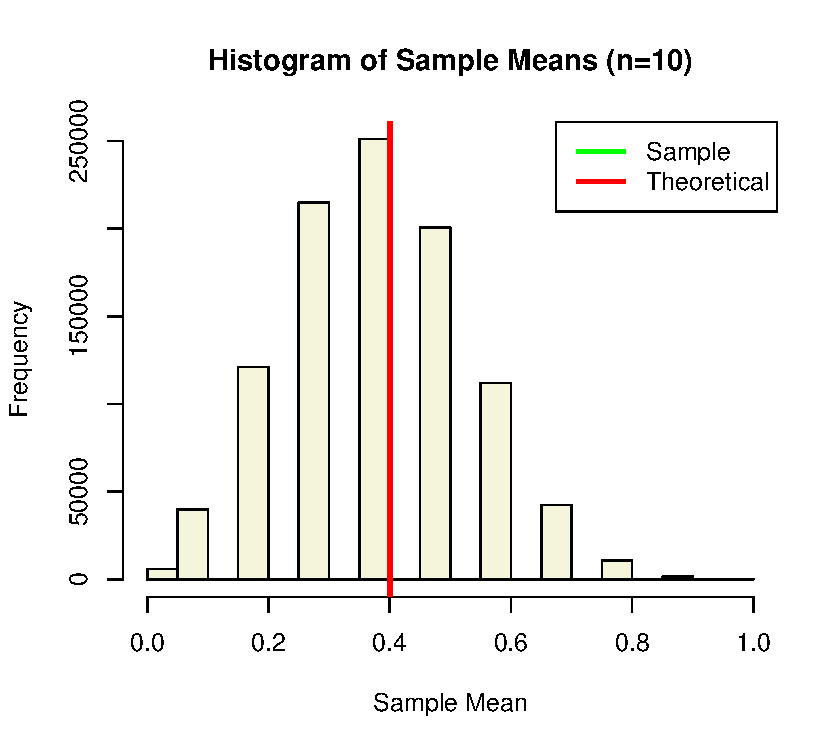
\includegraphics[height=.8\textheight]{clt10}
\end{center}
\end{frame}


\begin{frame}[fragile]{LLN Illustration}
\begin{lstlisting}
clt_function(20,.4)
\end{lstlisting}
\begin{center}
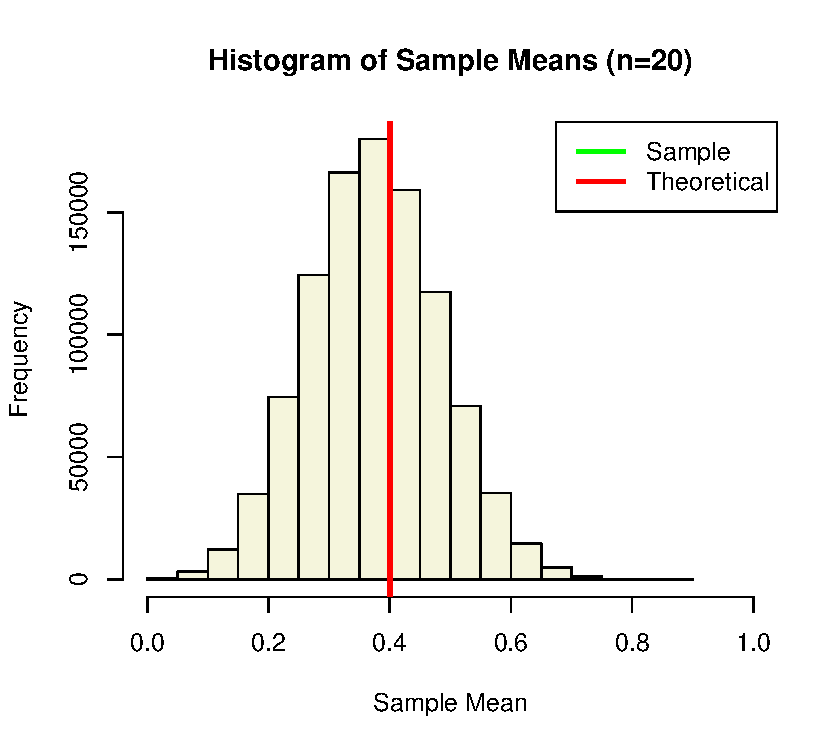
\includegraphics[height=.8\textheight]{clt20}
\end{center}
\end{frame}


\begin{frame}[fragile]{LLN Illustration}
\begin{lstlisting}
clt_function(100,.4)
\end{lstlisting}
\begin{center}
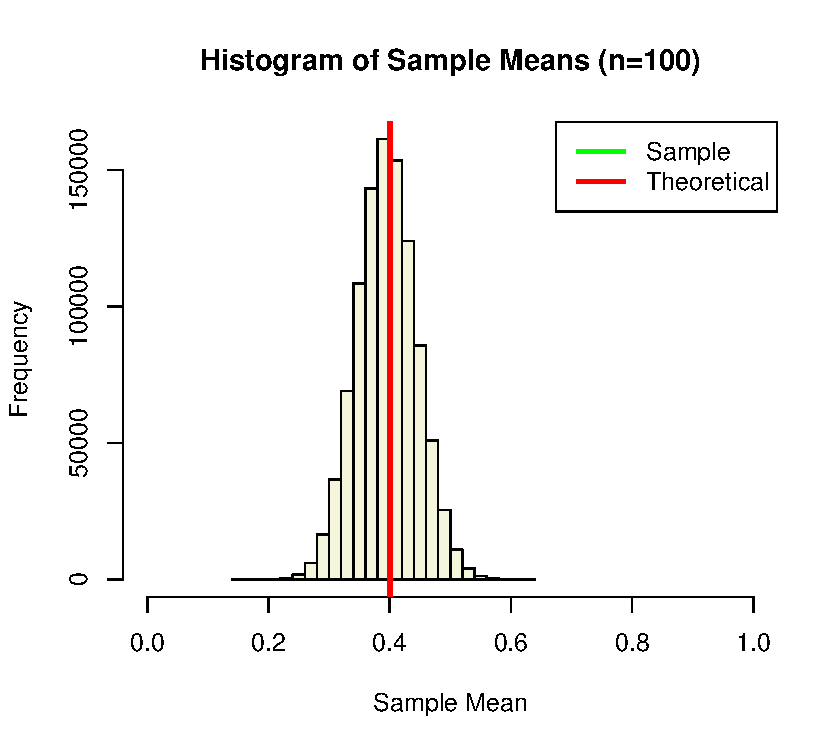
\includegraphics[height=.8\textheight]{clt100}
\end{center}
\end{frame}

\begin{frame}[fragile]{LLN Illustration}
\begin{lstlisting}
clt_function(1000,.4)
\end{lstlisting}
\begin{center}
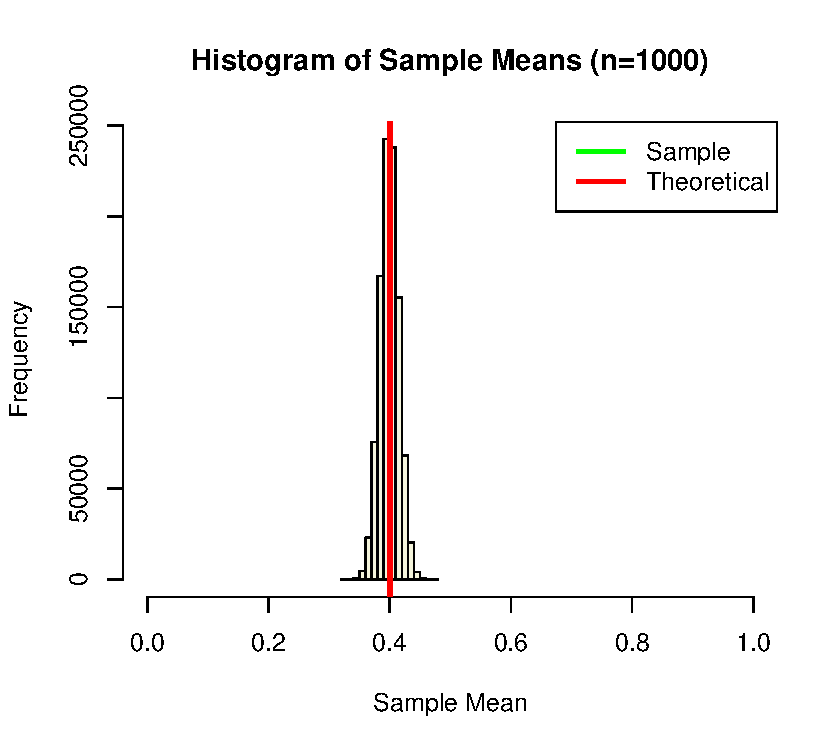
\includegraphics[height=.8\textheight]{clt1000}
\end{center}
\end{frame}




\begin{frame}[fragile]{CLT Illustration}
\begin{lstlisting}
clt_function_scaled <- function(n_sample,p){
  # create an empty vector for the means binomial samples
  clt <- NULL
  n <- n_sample   # sample size for each simulation
  # take the mean ofsamples of the uniform distribution. repeat 1,000 times
  for (i in 1:1000) {
    clt <-  c(clt, (rbinom(1000,n_sample,p)/n_sample-p)*sqrt(n_sample))
  }
  theoretical_mean <- 0
  hist(clt, xlim=c(-3, 3), xlab='Sample Mean', main=paste0("Histogram of Standardized Sample Means (n=", eval(n_sample),")"), col='beige')
  abline(v=mean(clt), lwd=3, col='green')
  abline(v=theoretical_mean, lwd=3, col='red')
  legend(c("Sample", "Theoretical"),x='topright', lwd=c(3,3), col=c('green', 'red'))
}
\end{lstlisting}
\end{frame}

\begin{frame}[fragile]{CLT Illustration}
\begin{lstlisting}
clt_function_scaled(10,.4)
\end{lstlisting}
\begin{center}
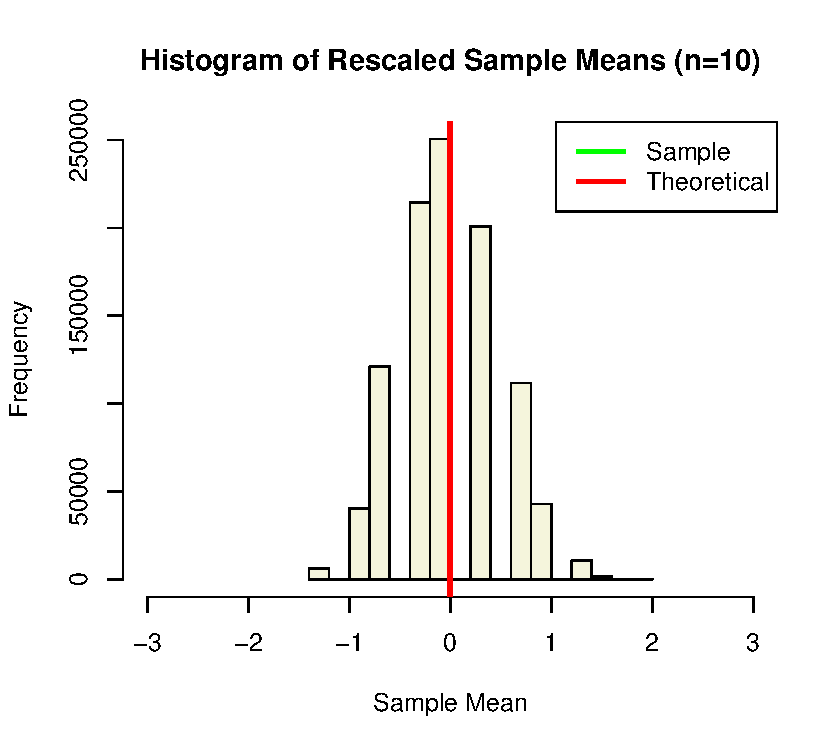
\includegraphics[height=.8\textheight]{clts10}
\end{center}
\end{frame}


\begin{frame}[fragile]{CLT Illustration}
\begin{lstlisting}
clt_function_scaled(20,.4)
\end{lstlisting}
\begin{center}
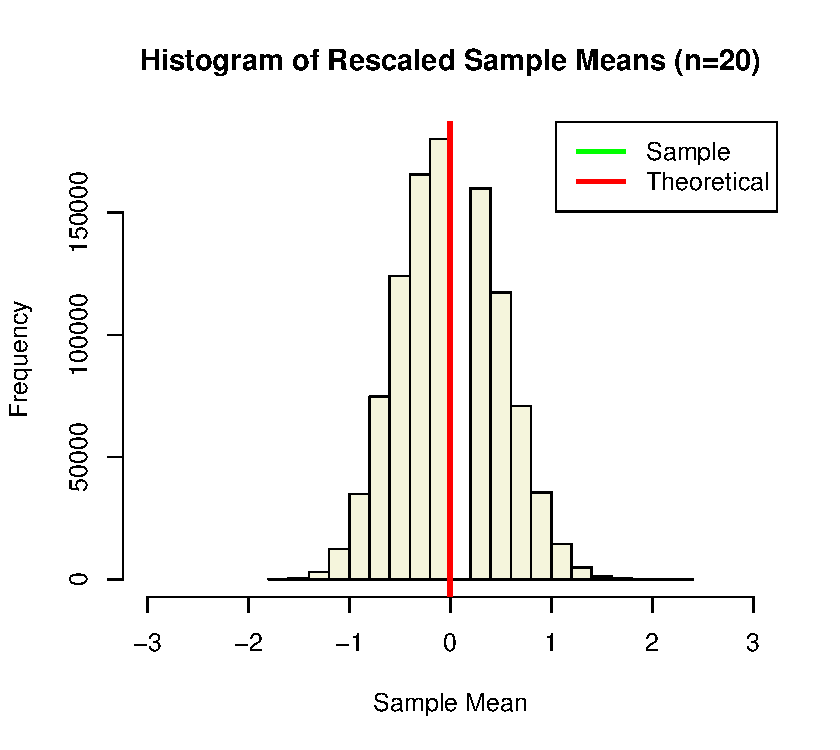
\includegraphics[height=.8\textheight]{clts20}
\end{center}
\end{frame}



\begin{frame}[fragile]{CLT Illustration}
\begin{lstlisting}
clt_function_scaled(100,.4)
\end{lstlisting}
\begin{center}
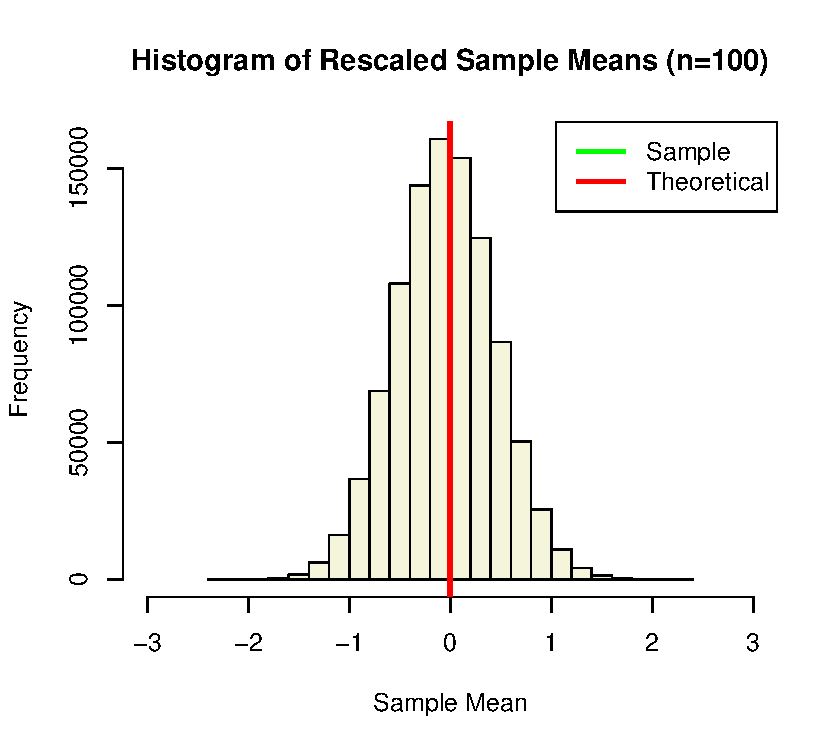
\includegraphics[height=.8\textheight]{clts100}
\end{center}
\end{frame}


\begin{frame}[fragile]{CLT Illustration}
\begin{lstlisting}
clt_function_scaled(1000,.4)
\end{lstlisting}
\begin{center}
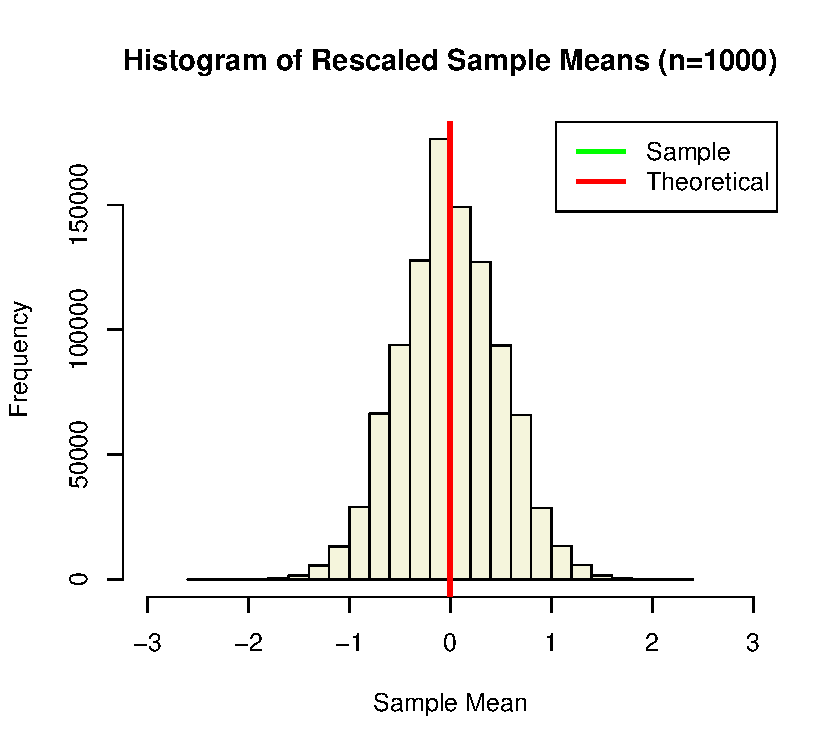
\includegraphics[height=.8\textheight]{clts1000}
\end{center}
\end{frame}




\begin{frame}{CLT interpretation}
 \[
\bar{X}_{N}\sim\mathcal{N}\left(\mu,\frac{\sigma^{2}}{N}\right)
\]
\begin{itemize}

	\item This is {\bf not strictly correct}: the CLT just tells us that $\bar{X}_{N}$ will be approximately
			 distributed  $\mathcal{N}\left(\mu,\frac{\sigma^{2}}{N}\right)$ as $N$ gets large,
			but in any finite sample the distribution of $\bar{X}_{N}$
	\begin{itemize}
		\item might not be centered around $\mu$
		\item might not have variance $\sigma^2/N$
		\item might not be normal
	\end{itemize}

	\item for i.i.d. normal case, the above statement actually is strictly correct. 

	\item In empirical economics, we generally use this approximation, but it's important to keep
			in mind that it's not always a good approximation, particularly for small sample sizes when
			the underlying distribution of the random variable is not itself normal.
\end{itemize}
\end{frame}


\begin{frame}{CLT extensions}

\begin{itemize}
	\item Like the LLN, there are versions of the CLT that get away from both the {\bf identical} and {\bf independent}
			aspects of the version we presented. But we \emph{do} need related conditions. See: {\bf ergodicity}, 
			{\bf stationarity}, {\bf weak dependence}.
\end{itemize}
\end{frame}



\begin{frame}{Finite sample distributions}
\begin{itemize}
	\item It is typically difficult to say much about the distributions of statistics 
			in {\bf finite samples}.

	\smallskip
	\item Exception: when the underlying random variables are normally distributed. Note that
			above, it was trivial to derive the distribution of $\bar{X}_N$ when $X_i$ was
			i.i.d. normal.
			
	\smallskip
	\item {\bf Monte Carlo studies} (simulation studies) are typically used to explore 
			the finite-sample properties of estimators. 
			
	\smallskip
	\item We'll talk (briefly) later about {\bf bootstrapped standard errors},
			which can have appealing finite sample properties. 

\end{itemize}
\end{frame}


\begin{frame}{Multivariate extensions}
\begin{itemize}
	\item Let $\left\{{\bf X}_i\right\}$ for $i=1,2,\dots,\infty$ be an i.i.d. sequence of vectors of random variables
			with finite first and second moments. 
	\begin{itemize}		
		\item Note that here we're asking for the ${\bf X}_i$ vector to be i.i.d. across $i$. Different elements of
		${\bf X}_i$ need not be identical or independent. 
	\end{itemize}


	\item The extension of the LLN to {\bf multivariate} random variables is trivial. We can write\[
			{\bf \bar{X}}_N \overset{p}{\rightarrow} E\left( {\bf X}_i \right)
		\]
		
	\item The multivariate CLT holds that\[
		\sqrt{N} \left({\bf \bar{X}}_N - E\left( {\bf X}_i \right) \right) \overset{d}{\rightarrow} \mathcal{N} \left(0,\Sigma\right),
	\]
	where $\Sigma = E\left[\left({\bf X}_i - E\left( {\bf X}_i \right)\right)\left({\bf X}_i - E\left( {\bf X}_i \right)\right)'\right]$

\end{itemize}
\end{frame}


\begin{frame}{Using the CLT}

	\[
		\sqrt{N} \left( \bar{X}_N  - \mu\right) \overset{d}{\rightarrow} \mathcal{N}\left(0,\sigma^2\right) 
	\]

\begin{itemize}
	\item We typically use the CLT to estimate the (approximate) distribution of estimators.

	\medskip
	\item This means that we need an estimate of $\sigma^2$, and then $\sigma^2/N$ estimates
			the variance of $\bar{X}_N$

\end{itemize}
\end{frame}





\begin{frame}{Estimating variance}
\begin{itemize}
	\item Consider the usual setup with $X_i$ i.i.d. for $i=1,2,\dots,\infty$.

	\medskip
	\item Let's show that \[
			E\left[\left(X_i - \bar{X}_N \right)^2\right] = \sigma^2 \left(\frac{N-1}{N}\right)
		\]

	\medskip
	\item It follows that $E\left[s_N^2 \right] = \sigma^2$, where\[
s_N^2 \equiv \frac{1}{N-1}\sum_{i=1}^{N} \left(X_i - \bar{X}_N \right)^2
\]

	\medskip
	\item But also notice that for large $N$, there is little difference between this estimator and one that divides by $N$.

\end{itemize}
\end{frame}



\begin{frame}{Standard errors}
\[
s_N^2 \equiv \frac{1}{N-1}\sum_{i=1}^{N} \left(X_i - \bar{X}_N \right)^2
\]
\begin{itemize}
	\item We can estimate $Var\left(\bar{X}_N\right)=\frac{\sigma^2}{N}$ with $\frac{s^2}{N}$


	\item A {\bf standard error} refers to our estimate of $\sqrt{Var\left( \bar{X}_N \right)}$:\[
		\sqrt{\frac{s^2}{N}}
\]

	\item Given the {\bf asymptotic normality} of $\bar{X}_N$, these standard errors allow us to
			make statements about the (approximate) CDF of $\bar{X}_N$.
	

	\item Note that \emph{standard errors} refer to an estimate of the \emph{standard deviation}
			of an estimator.
\end{itemize}
\end{frame}





\end{document}